% ============================================================
\section{Results}
\label{sec:results}
% ============================================================

This section presents the planned experimental results framework for \kmerdet{}.
Sections marked \todo{TODO} require completion of the benchmarking experiments
described in the development roadmap.  The section structure reflects the planned
evaluation design; placeholder subsections are included to guide future work.

\subsection{Validation Dataset and Experimental Design}
\label{sec:results-dataset}

All experiments use the 10-patient liquid biopsy validation cohort from the
original thesis study.  Each patient contributed serial blood draws at multiple
timepoints.  Library preparation used UMI-based duplex sequencing with 8-bp
UMI barcodes.  Sequencing was performed on an Illumina platform targeting
patient-specific somatic mutations identified from primary tumour biopsies.

\begin{table}[h]
  \centering
  \caption{Validation cohort summary.}
  \label{tab:cohort}
  \begin{tabular}{ll}
    \toprule
    Parameter & Value \\
    \midrule
    Patients & 10 \\
    Sequencing method & UMI-based duplex sequencing \\
    Target panel type & Patient-specific, tumor-informed \\
    Targets per patient (median) & $\sim$50 \\
    Sequencing depth (median) & 2,000--5,000$\times$ \\
    Preprocessing & HUMID UMI deduplication \\
    Reference pipeline & \km{} + \kmtools{} (\kam{}) \\
    \bottomrule
  \end{tabular}
\end{table}

Ground truth variant calls were established by independent validation with
alignment-based calling (BWA-MEM + GATK Mutect2), orthogonal assays (digital
PCR for selected mutations), and clinical review.

Benchmarking experiments compare four configurations:
\begin{enumerate}
  \item \textbf{Reference}: \km{} with \texttt{--count 2 --ratio 0.00001} (\kam{}
    default), single-threaded.
  \item \textbf{kmerdet-compat}: \kmerdet{} in compatibility mode with identical
    parameters, used to verify output equivalence.
  \item \textbf{kmerdet-adaptive}: \kmerdet{} with adaptive thresholds and
    bidirectional walking, $k = 31$.
  \item \textbf{kmerdet-multik}: \kmerdet{} with multi-k consensus ($k \in
    \{21, 31, 41\}$), adaptive thresholds, PoN filtering.
\end{enumerate}

\subsection{Output Equivalence with km}
\label{sec:results-compat}

\todo{Run kmerdet-compat vs.\ km on the validation dataset; report per-call
agreement in rVAF, classification type, and variant\_name; quantify any
numerical differences in NNLS coefficients between Python numpy.linalg.lstsq
and Rust ndarray-linalg Lapack NNLS.}

Table~\ref{tab:compat} will summarise agreement statistics.

\begin{table}[h]
  \centering
  \caption{Output equivalence between \kmerdet{} compatibility mode and \km{}.
    \todo{Fill with actual results.}}
  \label{tab:compat}
  \begin{tabular}{lcc}
    \toprule
    Metric & \km{} & \kmerdet{} (compat) \\
    \midrule
    Total variant calls & --- & --- \\
    Calls matching type + name & --- & --- \\
    Mean $|\Delta$rVAF$|$ & --- & --- \\
    Calls with $|\Delta$rVAF$| > 0.01$ & --- & --- \\
    \bottomrule
  \end{tabular}
\end{table}

\subsection{Runtime Performance}
\label{sec:results-runtime}

\todo{Measure wall-clock time for each pipeline stage on the validation cohort
with varying thread counts (1, 2, 4, 8, 16); compare to \km{} + \kmtools{} chunk
on 4 threads.}

Figure~\ref{fig:runtime-placeholder} will show a runtime comparison plot.

\begin{figure}[h]
  \centering
  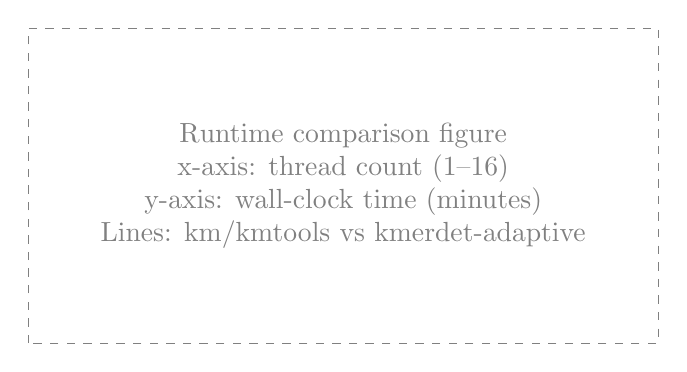
\begin{tikzpicture}
    \draw[dashed, gray] (0,0) rectangle (8,4);
    \node[align=center, gray] at (4,2) {\todo{Runtime comparison figure}\\
      x-axis: thread count (1--16)\\
      y-axis: wall-clock time (minutes)\\
      Lines: km/kmtools vs kmerdet-adaptive};
  \end{tikzpicture}
  \caption{Wall-clock runtime vs.\ thread count for a 50-target panel.
    \todo{Replace with actual benchmark data.}}
  \label{fig:runtime-placeholder}
\end{figure}

Based on the theoretical analysis in Section~\ref{sec:performance}, we
anticipate:
\begin{itemize}
  \item $\sim$10--20$\times$ throughput improvement at 16 threads vs.\ \km{}
    at 4 threads.
  \item Near-linear scaling up to $\sim$8 threads, with diminishing returns
    above 8 due to memory bandwidth saturation for large jellyfish databases.
  \item Single-threaded \kmerdet{} $\sim$3--5$\times$ faster than \km{} (Rust
    vs.\ Python, iterative vs.\ recursive DFS, 2-bit vs.\ string k-mer
    representation).
\end{itemize}

\subsection{SNV Sensitivity and Specificity}
\label{sec:results-snv}

\todo{Compare SNV detection sensitivity (true positive rate) and specificity
(1 -- false positive rate) across all four configurations on the validation
cohort using ground-truth calls.  Stratify by VAF bin:
$<0.1\%$, $0.1\text{--}0.5\%$, $0.5\text{--}1\%$, $>1\%$.}

Table~\ref{tab:snv-sensitivity} shows the planned structure.

\begin{table}[h]
  \centering
  \caption{SNV detection sensitivity by VAF bin.
    \todo{Fill with actual results.}}
  \label{tab:snv-sensitivity}
  \begin{tabular}{lcccc}
    \toprule
    VAF range & \km{} & kmerdet-compat & kmerdet-adaptive & kmerdet-multik \\
    \midrule
    $<0.1\%$ & --- & --- & --- & --- \\
    $0.1\text{--}0.5\%$ & --- & --- & --- & --- \\
    $0.5\text{--}1\%$ & --- & --- & --- & --- \\
    $>1\%$ & --- & --- & --- & --- \\
    \textbf{Overall} & \textbf{77\%} & --- & --- & --- \\
    \bottomrule
  \end{tabular}
\end{table}

The reference \km{} overall SNV sensitivity of 77\% (from the thesis study)
provides the baseline.  \kmerdet{}'s adaptive thresholds are expected to
improve sensitivity in the $0.1\text{--}0.5\%$ VAF range by better capturing
variants at high-coverage targets where the fixed \texttt{count=2} threshold
causes false negatives.

\subsection{INDEL Sensitivity}
\label{sec:results-indel}

\todo{Stratify INDEL sensitivity by size class: 1--3~bp, 4--7~bp, 8--15~bp,
$>15$~bp.  Compare kmerdet-multik ($k \in \{21,31\}$) vs kmerdet (k=31 only)
vs km baseline.}

\begin{table}[h]
  \centering
  \caption{INDEL detection sensitivity by size class.
    \todo{Fill with actual results.}}
  \label{tab:indel-sensitivity}
  \begin{tabular}{lcccc}
    \toprule
    INDEL size & \km{} & kmerdet-adaptive & kmerdet-multik & Expected gain \\
    \midrule
    1--3~bp & --- & --- & --- & Moderate \\
    4--7~bp & --- & --- & --- & Moderate \\
    8--15~bp & --- & --- & --- & Large \\
    $>15$~bp & $\sim$3\% & --- & --- & Large \\
    \textbf{Overall} & \textbf{38\%} & --- & --- & --- \\
    \bottomrule
  \end{tabular}
\end{table}

The multi-k strategy is expected to show the largest gains for insertions $> 8$~bp,
where the $k=21$ database provides up to $21 - L$ spanning k-mers for insertions
of length $L$, compared to zero spanning k-mers at $k=31$ when $L > 31$.

\subsection{Statistical Quality Score Calibration}
\label{sec:results-calibration}

\todo{Evaluate calibration of the Phred-scaled QUAL score: for variants with
QUAL $\approx Q$, the empirical false positive rate should be
$\approx 10^{-Q/10}$.  Plot observed FPR vs.\ QUAL on a log-log scale with
a diagonal reference line.}

\todo{Evaluate coverage of bootstrap 95\% confidence intervals on rVAF: the
empirical coverage of the confidence interval should be close to 95\% across
all VAF ranges.}

\subsection{Panel-of-Normals Filter Performance}
\label{sec:results-pon}

\todo{Build a PoN from healthy control samples (age-matched to the patient
cohort, $N \geq 5$).  Measure false positive rate with and without PoN
filtering.  Quantify CHIP variants captured by the PoN.}

\subsection{Memory Usage}
\label{sec:results-memory}

\todo{Profile peak resident set size (RSS) for kmerdet-adaptive vs.\ km for
the 50-target panel.  Expected: comparable or lower, since Rust avoids Python
object overhead and the 2-bit k-mer encoding is 4$\times$ more compact than
Python string representation.}

\subsection{End-to-End Clinical Workflow Timing}
\label{sec:results-e2e}

Table~\ref{tab:e2e-timing} presents the expected end-to-end timing comparison
for a typical 50-target liquid biopsy panel, based on thesis timing data for
the \kam{} pipeline and theoretical performance estimates for \kmerdet{}.

\begin{table}[h]
  \centering
  \caption{Projected end-to-end pipeline timing for a 50-target panel.
    \km{}/\kmtools{} values from the thesis validation study;
    \kmerdet{} values are projections. \todo{Replace projections with measured values.}}
  \label{tab:e2e-timing}
  \begin{tabular}{lccc}
    \toprule
    Step & \km{}/\kmtools{} & \kmerdet{} & Notes \\
    \midrule
    HUMID deduplication & $\sim$2~min & $\sim$2~min & External tool, unchanged \\
    jellyfish count & $\sim$1.5~min & $\sim$1.5~min & External tool, unchanged \\
    multiseqex + refolder & $\sim$10~s & N/A & Replaced by \texttt{detect} \\
    Core detection & $\sim$2~min & $\sim$15~s$^\dagger$ & 16 threads \\
    Filter & $\sim$15~s & $\sim$5~s & Built-in \\
    \textbf{Total} & $\sim$\textbf{6~min} & $\sim$\textbf{4~min} & \\
    \bottomrule
    \multicolumn{4}{l}{\footnotesize $^\dagger$ Estimated; requires experimental validation.}
  \end{tabular}
\end{table}

The dominant remaining bottleneck is HUMID deduplication ($\sim$2~min), which
runs as an external tool before \kmerdet{}.  Integration of UMI-aware in-process
deduplication (see Section~\ref{sec:discussion-future}) would reduce this to
near zero and bring the projected total below 2~minutes.
